
\documentclass{article}
\usepackage[margin=1in]{geometry}
\usepackage{amsmath}
\usepackage{amssymb}
\usepackage{graphicx}
\usepackage{tikz}
\usepackage{tcolorbox}
\usepackage{enumitem}
\usepackage{hyperref}
\usepackage{xcolor}
\usepackage{mdframed}

\newcommand{\slidenote}[1]{\begin{mdframed}[backgroundcolor=blue!10, linewidth=0pt]
\textbf{Slide Note:} #1
\end{mdframed}}

\newcommand{\lecturenote}[1]{\begin{mdframed}[backgroundcolor=green!10, linewidth=0pt]
\textbf{Lecture Note:} #1
\end{mdframed}}

\newcommand{\insight}[1]{\begin{mdframed}[backgroundcolor=yellow!10, linewidth=0pt]
\textbf{Key Insight:} #1
\end{mdframed}}

\title{Linear Boundaries for Binary Classification\\
\large A Comprehensive Study Guide}
\author{Machine Learning Course}
\date{}

\begin{document}

\maketitle

\begin{abstract}
This document provides a comprehensive explanation of linear boundaries for binary classification, synthesizing material from both lecture slides and the corresponding transcript. It covers the geometric intuition behind linear classifiers, their mathematical formulation in both two and higher dimensions, and lays the groundwork for understanding the perceptron algorithm. The material is organized to build intuition progressively while maintaining mathematical rigor.
\end{abstract}

\tableofcontents

\section{Introduction and Context}

\slidenote{We've covered regression and conditional probability estimation, both reformulated as optimization tasks. Now we'll apply optimization to classification.}

\lecturenote{We have spent a little bit of time talking about regression and conditional probability estimation. And in each case, we approach the learning problem by reformulating it as an optimization task. Now, let's circle back round to classification and bring the same optimization mindset to it.}

Classification is a fundamental task in machine learning where we aim to assign discrete labels to data points. In this study guide, we focus specifically on binary classification using linear boundaries—one of the most elegant and foundational approaches in machine learning.

\insight{The power of the optimization mindset in machine learning is that it provides a unified framework for approaching seemingly different problems like regression and classification.}

\section{Geometric Intuition of Linear Classification}

\subsection{Linear Decision Boundaries in Two Dimensions}

\slidenote{Decision boundary in 2D space with y-intercept = 4, slope = -4/3}

Let's begin with a concrete example in two dimensions to build intuition. Consider a 2D feature space where each point has coordinates $(x_1, x_2)$.

\begin{figure}[h]
\centering
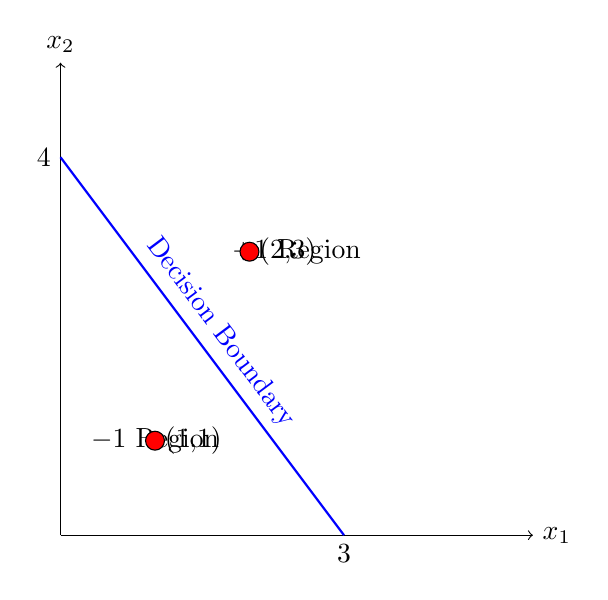
\begin{tikzpicture}[scale=1.2]
    \draw[->] (0,0) -- (5,0) node[right] {$x_1$};
    \draw[->] (0,0) -- (0,5) node[above] {$x_2$};
    \draw[thick, blue] (0,4) -- (3,0) node[midway, above, sloped] {Decision Boundary};
    \node at (2.5,3) {$+1$ Region};
    \node at (1,1) {$-1$ Region};
    \draw[fill=red] (2,3) circle (0.1) node[right] {(2,3)};
    \draw[fill=red] (1,1) circle (0.1) node[right] {(1,1)};
    \node[below] at (3,0) {3};
    \node[left] at (0,4) {4};
\end{tikzpicture}
\caption{A linear decision boundary in 2D space with positive and negative regions}
\end{figure}

\lecturenote{Let's start with a quick review of the geometry of linear classification. So here, we have a decision boundary in two dimensions. What is the formula for this boundary? Let's go ahead and derive that.}

The equation of this line can be derived as follows:
\begin{align}
    x_2 &= -\frac{4}{3}x_1 + 4 \quad \text{(slope-intercept form)}
\end{align}

We can rearrange this to get the standard form:
\begin{align}
    \frac{4}{3}x_1 + x_2 - 4 &= 0\\
    \Rightarrow 4x_1 + 3x_2 - 12 &= 0 \quad \text{(multiplied by 3)}
\end{align}

\insight{Linear decision boundaries will always be expressed in the form of a linear function equal to zero. This standardization simplifies both the mathematical analysis and implementation.}

\subsection{Making Predictions with Linear Boundaries}

Once we have the equation of the decision boundary, how do we use it to classify points? The key insight is that the linear function divides the space into two regions:

\begin{itemize}
    \item Points where the function evaluates to positive values
    \item Points where the function evaluates to negative values
\end{itemize}

\slidenote{For point (2,3): $4(2) + 3(3) - 12 = 8 + 9 - 12 = 5 > 0 \Rightarrow$ Predict +1}

Let's evaluate our linear function $f(x) = 4x_1 + 3x_2 - 12$ at the point $(2,3)$:
\begin{align}
    f(2,3) &= 4(2) + 3(3) - 12\\
    &= 8 + 9 - 12\\
    &= 5
\end{align}

Since $f(2,3) > 0$, we classify this point as $+1$.

\slidenote{For point (1,1): $4(1) + 3(1) - 12 = 4 + 3 - 12 = -5 < 0 \Rightarrow$ Predict -1}

Similarly, for the point $(1,1)$:
\begin{align}
    f(1,1) &= 4(1) + 3(1) - 12\\
    &= 4 + 3 - 12\\
    &= -5
\end{align}

Since $f(1,1) < 0$, we classify this point as $-1$.

\begin{tcolorbox}[colback=blue!5!white,colframe=blue!75!black,title=Classification Rule]
For a linear function $f(x) = w_1x_1 + w_2x_2 + \ldots + w_dx_d + b$:
\begin{itemize}
    \item If $f(x) > 0$, classify as $+1$
    \item If $f(x) < 0$, classify as $-1$
    \item If $f(x) = 0$, the point lies exactly on the decision boundary
\end{itemize}
\end{tcolorbox}

\lecturenote{At any given point, the way we make a prediction is to just plug the point into this linear function. If the result is positive, we predict plus one. If the result is negative, we predict minus one. It's very simple.}

\section{Generalization to D-Dimensional Space}

\subsection{Mathematical Formulation}

While the 2D case is easy to visualize, the real power of linear classification comes from its ability to generalize to higher dimensions.

\slidenote{Data points $\mathbf{x} \in \mathbb{R}^d$, Labels $y \in \{-1, +1\}$}

In the general case:
\begin{itemize}
    \item Data points are vectors in $d$-dimensional space: $\mathbf{x} \in \mathbb{R}^d$
    \item Labels remain binary: $y \in \{-1, +1\}$
\end{itemize}

\slidenote{Linear classifier defined by weight vector $\mathbf{w} \in \mathbb{R}^d$ and offset/bias $b \in \mathbb{R}$}

A linear classifier in $d$ dimensions is defined by:
\begin{itemize}
    \item A weight vector $\mathbf{w} = (w_1, w_2, \ldots, w_d) \in \mathbb{R}^d$
    \item A bias term (or offset) $b \in \mathbb{R}$
\end{itemize}

The decision boundary is the hyperplane defined by:
\begin{align}
    \mathbf{w} \cdot \mathbf{x} + b = 0
\end{align}

where $\mathbf{w} \cdot \mathbf{x} = w_1x_1 + w_2x_2 + \ldots + w_dx_d$ is the dot product.

\lecturenote{A linear classifier is now given by a vector, W, a D dimensional vector, as well as an offset b. The form of the boundary is w . x plus b equals zero.}

\insight{The dot product $\mathbf{w} \cdot \mathbf{x}$ can be interpreted geometrically as the projection of $\mathbf{x}$ onto the direction of $\mathbf{w}$, scaled by the magnitude of $\mathbf{w}$. The bias term $b$ shifts the decision boundary away from the origin.}

\subsection{Prediction Rule in Higher Dimensions}

The prediction rule generalizes naturally from the 2D case:

\begin{align}
    \hat{y} = \begin{cases}
    +1 & \text{if } \mathbf{w} \cdot \mathbf{x} + b > 0\\
    -1 & \text{if } \mathbf{w} \cdot \mathbf{x} + b < 0
    \end{cases}
\end{align}

This can be written more compactly using the sign function:
\begin{align}
    \hat{y} = \text{sign}(\mathbf{w} \cdot \mathbf{x} + b)
\end{align}

\lecturenote{And in when we wanna make a prediction on a new point x, we simply compute the linear function, and then look at the sign of the outcome. If it's positive, we predict plus one. If it's negative, we predict minus one.}

\subsection{Correctness Condition}

How do we know if our prediction is correct? Let $y$ be the true label of a point $\mathbf{x}$.

\slidenote{Prediction is correct if and only if: True label $y = +1$ and $\mathbf{w} \cdot \mathbf{x} + b > 0$, OR True label $y = -1$ and $\mathbf{w} \cdot \mathbf{x} + b < 0$}

Our prediction is correct if and only if one of these conditions holds:
\begin{itemize}
    \item $y = +1$ and $\mathbf{w} \cdot \mathbf{x} + b > 0$
    \item $y = -1$ and $\mathbf{w} \cdot \mathbf{x} + b < 0$
\end{itemize}

\slidenote{Compact form: $y(\mathbf{w} \cdot \mathbf{x} + b) > 0$}

These conditions can be combined into a single, elegant expression:
\begin{align}
    y(\mathbf{w} \cdot \mathbf{x} + b) > 0
\end{align}

\lecturenote{A more compact way to write this is simply to say that the true label, times w . x plus b should be greater than zero. That is either both of these things are positive, or both of them are negative. So instead of having two conditions like we have over here, we just have a single compact condition, and we are gonna make heavy use of this particular formulation.}

\insight{This compact formulation is not just mathematically elegant—it will be the foundation for the perceptron algorithm and many other classification methods. It effectively measures whether the prediction has the same sign as the true label.}

\section{Geometric Interpretation}

To deepen our understanding, let's explore the geometric interpretation of linear classification:

\begin{itemize}
    \item The weight vector $\mathbf{w}$ is perpendicular (normal) to the decision boundary hyperplane
    \item The magnitude of $\mathbf{w}$ doesn't affect the orientation of the boundary, only its scale
    \item The bias term $b$ determines how far the hyperplane is from the origin
    \item The signed distance from a point $\mathbf{x}$ to the decision boundary is proportional to $\frac{\mathbf{w} \cdot \mathbf{x} + b}{||\mathbf{w}||}$
\end{itemize}

\begin{figure}[h]
\centering
\begin{tikzpicture}[scale=1.2]
    \draw[->] (0,0) -- (5,0) node[right] {$x_1$};
    \draw[->] (0,0) -- (0,5) node[above] {$x_2$};
    \draw[thick, blue] (0,4) -- (3,0) node[midway, above, sloped] {$\mathbf{w} \cdot \mathbf{x} + b = 0$};
    \draw[->, thick, red] (1.5,2) -- (2.5,3.33) node[right] {$\mathbf{w}$};
    \node at (2.5,3) {$+1$ Region};
    \node at (1,1) {$-1$ Region};
\end{tikzpicture}
\caption{Geometric interpretation of the weight vector $\mathbf{w}$ as normal to the decision boundary}
\end{figure}

\section{Connection to the Perceptron Algorithm}

\slidenote{We'll use this formulation to develop the perceptron algorithm—one of the most influential algorithms for linear classification.}

The formulation we've developed provides the foundation for the perceptron algorithm, which is one of the earliest and most influential algorithms for linear classification.

\lecturenote{What we'll be doing next is to use this formulation to write down one of the most beautiful and influential algorithms for linear classification, the perceptron.}

The perceptron algorithm:
\begin{itemize}
    \item Iteratively updates the weight vector $\mathbf{w}$ and bias $b$ based on misclassified points
    \item Uses the correctness condition $y(\mathbf{w} \cdot \mathbf{x} + b) > 0$ to identify misclassifications
    \item Converges to a solution if the data is linearly separable (i.e., if a perfect linear boundary exists)
\end{itemize}

\insight{The perceptron algorithm is not just historically significant—it forms the conceptual foundation for neural networks and deep learning. A modern neural network can be viewed as multiple layers of perceptron-like units with non-linear activation functions.}

\section{Practice Problems}

To solidify your understanding, try these practice problems:

\begin{tcolorbox}[colback=gray!10, colframe=gray!50!black, title=Problem 1]
Consider the linear boundary $2x_1 - 3x_2 + 6 = 0$ in 2D space.
\begin{enumerate}[label=(\alph*)]
    \item Sketch this boundary.
    \item Determine which side corresponds to the positive region.
    \item Classify the points $(1,2)$, $(3,1)$, and $(0,0)$.
\end{enumerate}
\end{tcolorbox}

\begin{tcolorbox}[colback=gray!10, colframe=gray!50!black, title=Problem 2]
For a linear classifier in 3D with $\mathbf{w} = (1, 2, -1)$ and $b = -3$:
\begin{enumerate}[label=(\alph*)]
    \item Write the equation of the decision boundary.
    \item Classify the points $(2,1,0)$, $(1,0,1)$, and $(0,0,0)$.
    \item Is the point $(1,1,1)$ correctly classified if its true label is $-1$?
\end{enumerate}
\end{tcolorbox}

\begin{tcolorbox}[colback=gray!10, colframe=gray!50!black, title=Problem 3]
Prove that scaling the weight vector $\mathbf{w}$ and bias $b$ by the same positive constant does not change the predictions of a linear classifier.
\end{tcolorbox}

\section{Summary and Key Takeaways}

\begin{itemize}
    \item Linear classification uses a hyperplane to separate data into two classes
    \item In 2D, the decision boundary is a line; in higher dimensions, it's a hyperplane
    \item A linear classifier is defined by a weight vector $\mathbf{w}$ and bias $b$
    \item The decision rule is based on the sign of $\mathbf{w} \cdot \mathbf{x} + b$
    \item A prediction is correct when $y(\mathbf{w} \cdot \mathbf{x} + b) > 0$
    \item This formulation is the foundation for the perceptron algorithm
\end{itemize}

\insight{Linear classification, despite its simplicity, remains a powerful tool in machine learning. It provides excellent interpretability, computational efficiency, and serves as a building block for more complex models. Understanding linear boundaries thoroughly is essential for mastering more advanced classification techniques.}

\section{Further Reading}

\begin{itemize}
    \item The Perceptron Algorithm and its convergence properties
    \item Support Vector Machines: Optimal linear boundaries with maximum margin
    \item Logistic Regression: Probabilistic interpretation of linear boundaries
    \item Neural Networks: From perceptrons to deep learning
\end{itemize}

\end{document}
